\section{Architecture}

The main actors in the system are clear: the heart of the problem is the temperature-sensitive cargo that needs to be transported. This cargo is loaded in the refrigerated containers, also known as reefers. Each type of cargo requires different temperature and air composition, so these settings differ among the reefers. There is at least one temperature sensor and one gas monitoring sensor in every reefer. Reefers, together with regular containers and other cargo are loaded onto a vessel and transported across the sea.

When the temperature and the air quality are monitored, the goal is to transfer the data to:
\begin{itemize}
    \item \textit{Collection point/database}, so that the transport company can prove to its customers that the cargo maintained the desired temperature throughout the whole duration of the journey. Some systems allow the customer to monitor the data from the container in real time.
    \item \textit{Ship bridge}, to ensure that the temperature in the container is not too high (i.e. due to a power loss) and that the systems are operating normally (i.e. there is no fire in the container). 
\end{itemize}

The simplest architecture for this transfer of data from every container would probably consist of sensors submitting data directly to the collection point. This architecture is illustrated in Figure \ref{fig:arch-ver1}. It is obvious that this probably has many drawbacks. Even if there are only two sensors in each containers, there are still hundreds of containers on a ship. If there was only one collection point for all of Maersk’s fleet, this point would need to handle connections from tens of thousands devices, since there are hundreds of ships in operation worldwide.

\begin{figure}[ht]
    \centering
    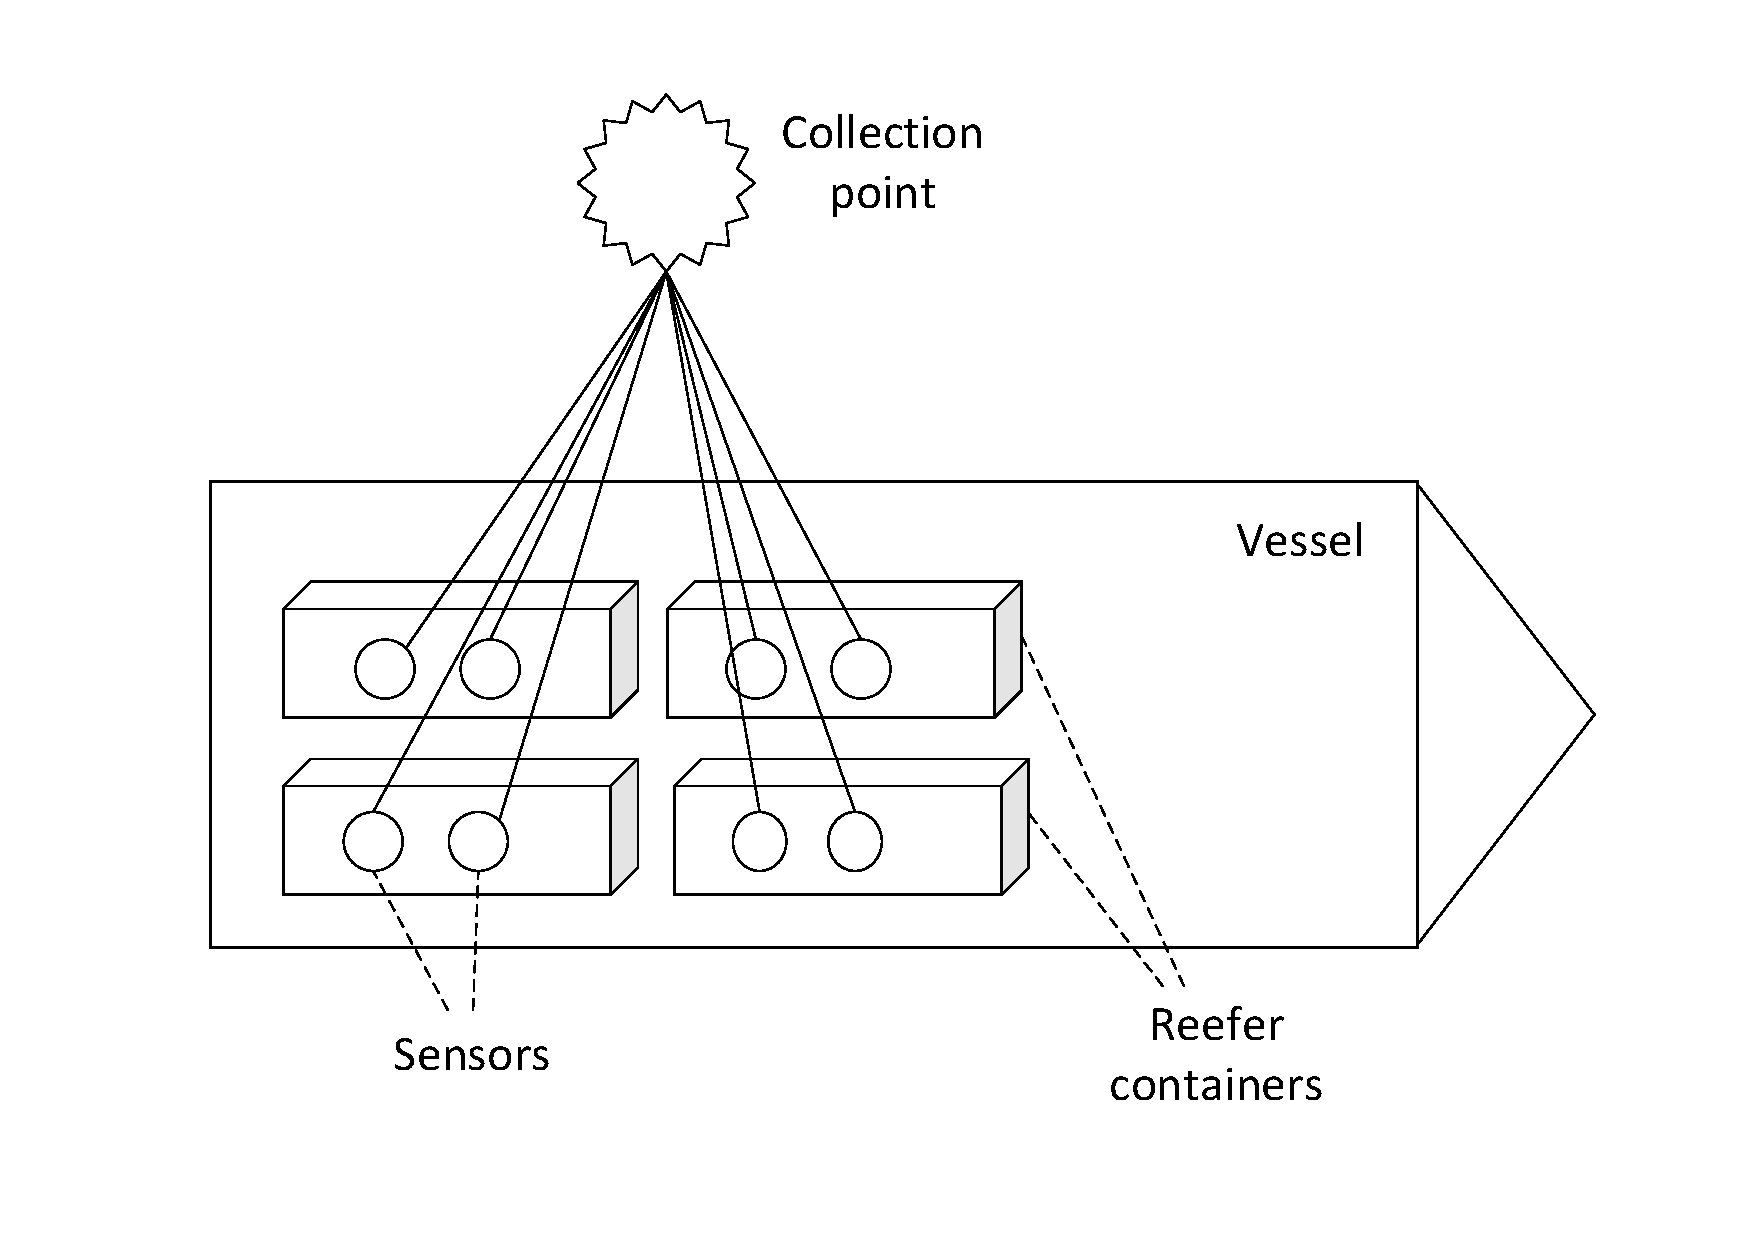
\includegraphics[width=0.8\textwidth]{00images/arch-ver1}
    \caption{Simplest version of the architecture. Each sensor communicates directly with the collection point.}
    \label{fig:arch-ver1}
\end{figure}

A solution to this problem is to introduce a \textit{hub}. Hub is a cluster node, that collects, processes and re-transmits data to the sink, but it does not sense any data by itself. The sensors in the container would connect to a hub and the hub would then connect to sink. This architecture is illustrated in Figure \ref{fig:arch-ver2}. Such architecture reduces the number of connections that need to be handled by the sink and also limits the necessary transmission power of the sensor. The problem then lies in the relative position of the hub. If the hub is positioned too close to the sensors, we can lower the necessary transmission power of the sensors, but more hubs per vessel would be needed to cover all of the containers. If the hub is too far from the sensors, less hubs per vessel would be needed, but the range of the sensors would need to increase. The lesser the hubs are there, the fewer communication links to the sink are needed. In a shipping scenario, where vessels are often out of reach of the traditional \acrshort{gsm} band and satellite communication must be used to transmit data to shore. Satellite link is a scarce resource and limiting the amount of satellite connections required is beneficial.

\begin{figure}[ht]
    \centering
    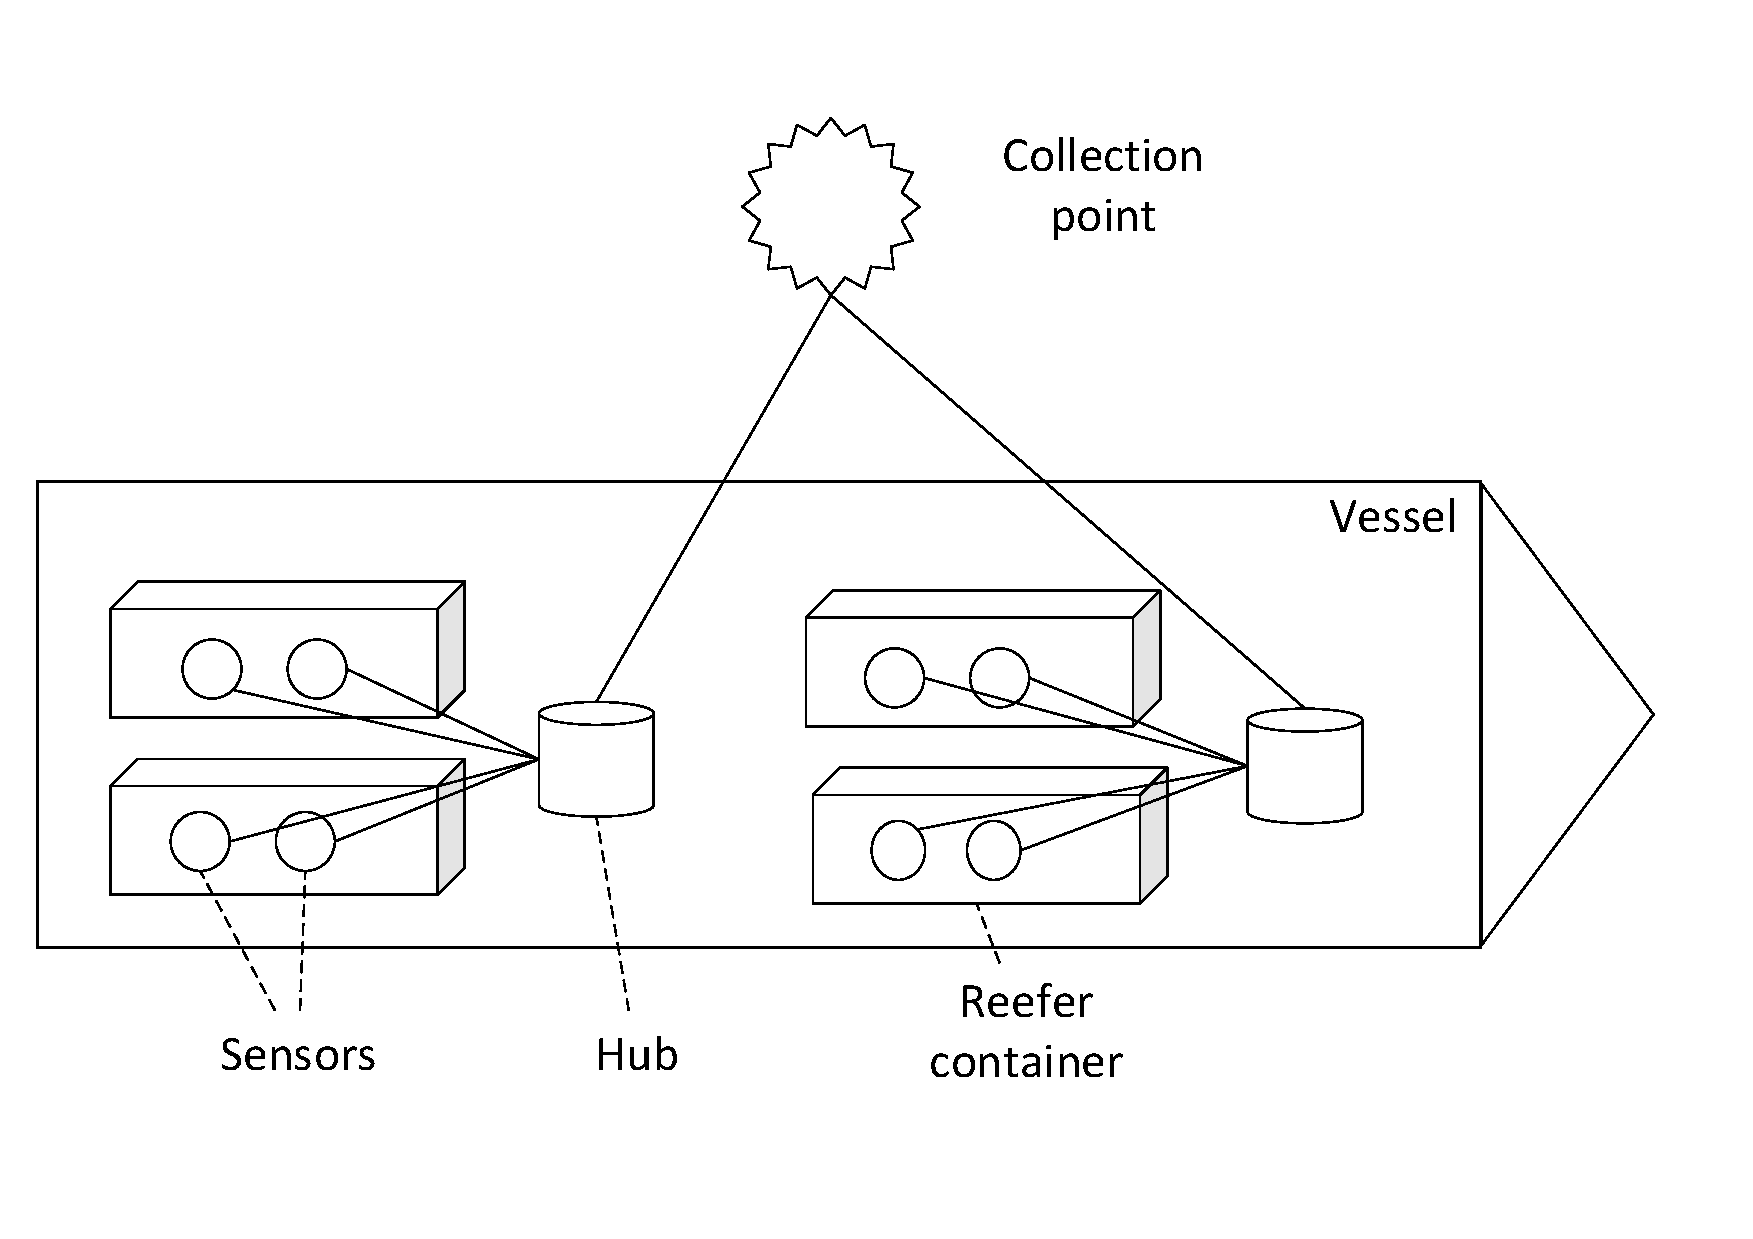
\includegraphics[width=0.8\textwidth]{00images/arch-ver2}
    \caption{Slightly improved version of the architecture. Sensors communicate with an on-board hub. Hubs then communicate with the collection point. }
    \label{fig:arch-ver2}
\end{figure}

An alternative solution to compromise between the sensor transmit power and number of hubs required, is to introduce a second-level hub. Second-level hubs are the middle man between first-level hubs and the sink. Sensors connect and transfer their data to the first-level hub. This hub processes the data and forwards it to the second-level hub. Second-level hub collects the data and forwards them to the sink in batches. A plausible placements of the hubs could be inside a container for the first-level hub and on the bridge for the second-level hub. In this setup, the sensors only need to transmit their data over a short distance, therefore the power consumption can be reduced. The second-level hub collects data from the whole vessel before forwarding them to the sink. If there only is one second-level hub per vessel, the number of satellite links required is reduced.
%
% 
% \footnotetext{This does not neccessarily refer to the physical distance to the sensors, rather than relative position in the architecture with respect to}